\documentclass[11pt]{article}
\usepackage{graphicx}
\usepackage{cite}
\def\BibTeX{{\rm B\kern-.05em{\sc i\kern-.025em b}\kern-.08em
    T\kern-.1667em\lower.7ex\hbox{E}\kern-.125emX}}
\usepackage{url}
    \makeatletter
    \g@addto@macro{\UrlBreaks}{\UrlOrds}
    \makeatother
\usepackage{appendix}
\usepackage[version=3]{mhchem}
\usepackage{amsmath}
\usepackage{booktabs}
\renewcommand{\arraystretch}{1.2}
\usepackage{amssymb}
\usepackage{float}
\usepackage{commath}
\usepackage{siunitx}
\usepackage{multirow}
\usepackage[a4paper,margin=20mm]{geometry}
\setlength{\parskip}{\baselineskip}%
\setlength{\parindent}{0pt}%
\sisetup{detect-all}
\begin{document}
\title{\textbf{UCL Mechanical Engineering}\\MECH0015 TTT \& MVC Quiz Questions}
\author{Hasha Dar}
\maketitle
\section{Why does the tensile strength of a steel drop with carbon content after the eutectoid composition is reached?}
During cooling, we can form three different phases when we vary the carbon content around 0.8\%. Let us consider a case when we cool three samples with carbon content 0.4\% \ce{C}, 0.8\% \ce{C} and 1\% \ce{C} from \SI{900}{\celsius} to \SI{723}{\celsius}. 

\begin{figure}[H]
    \centering
    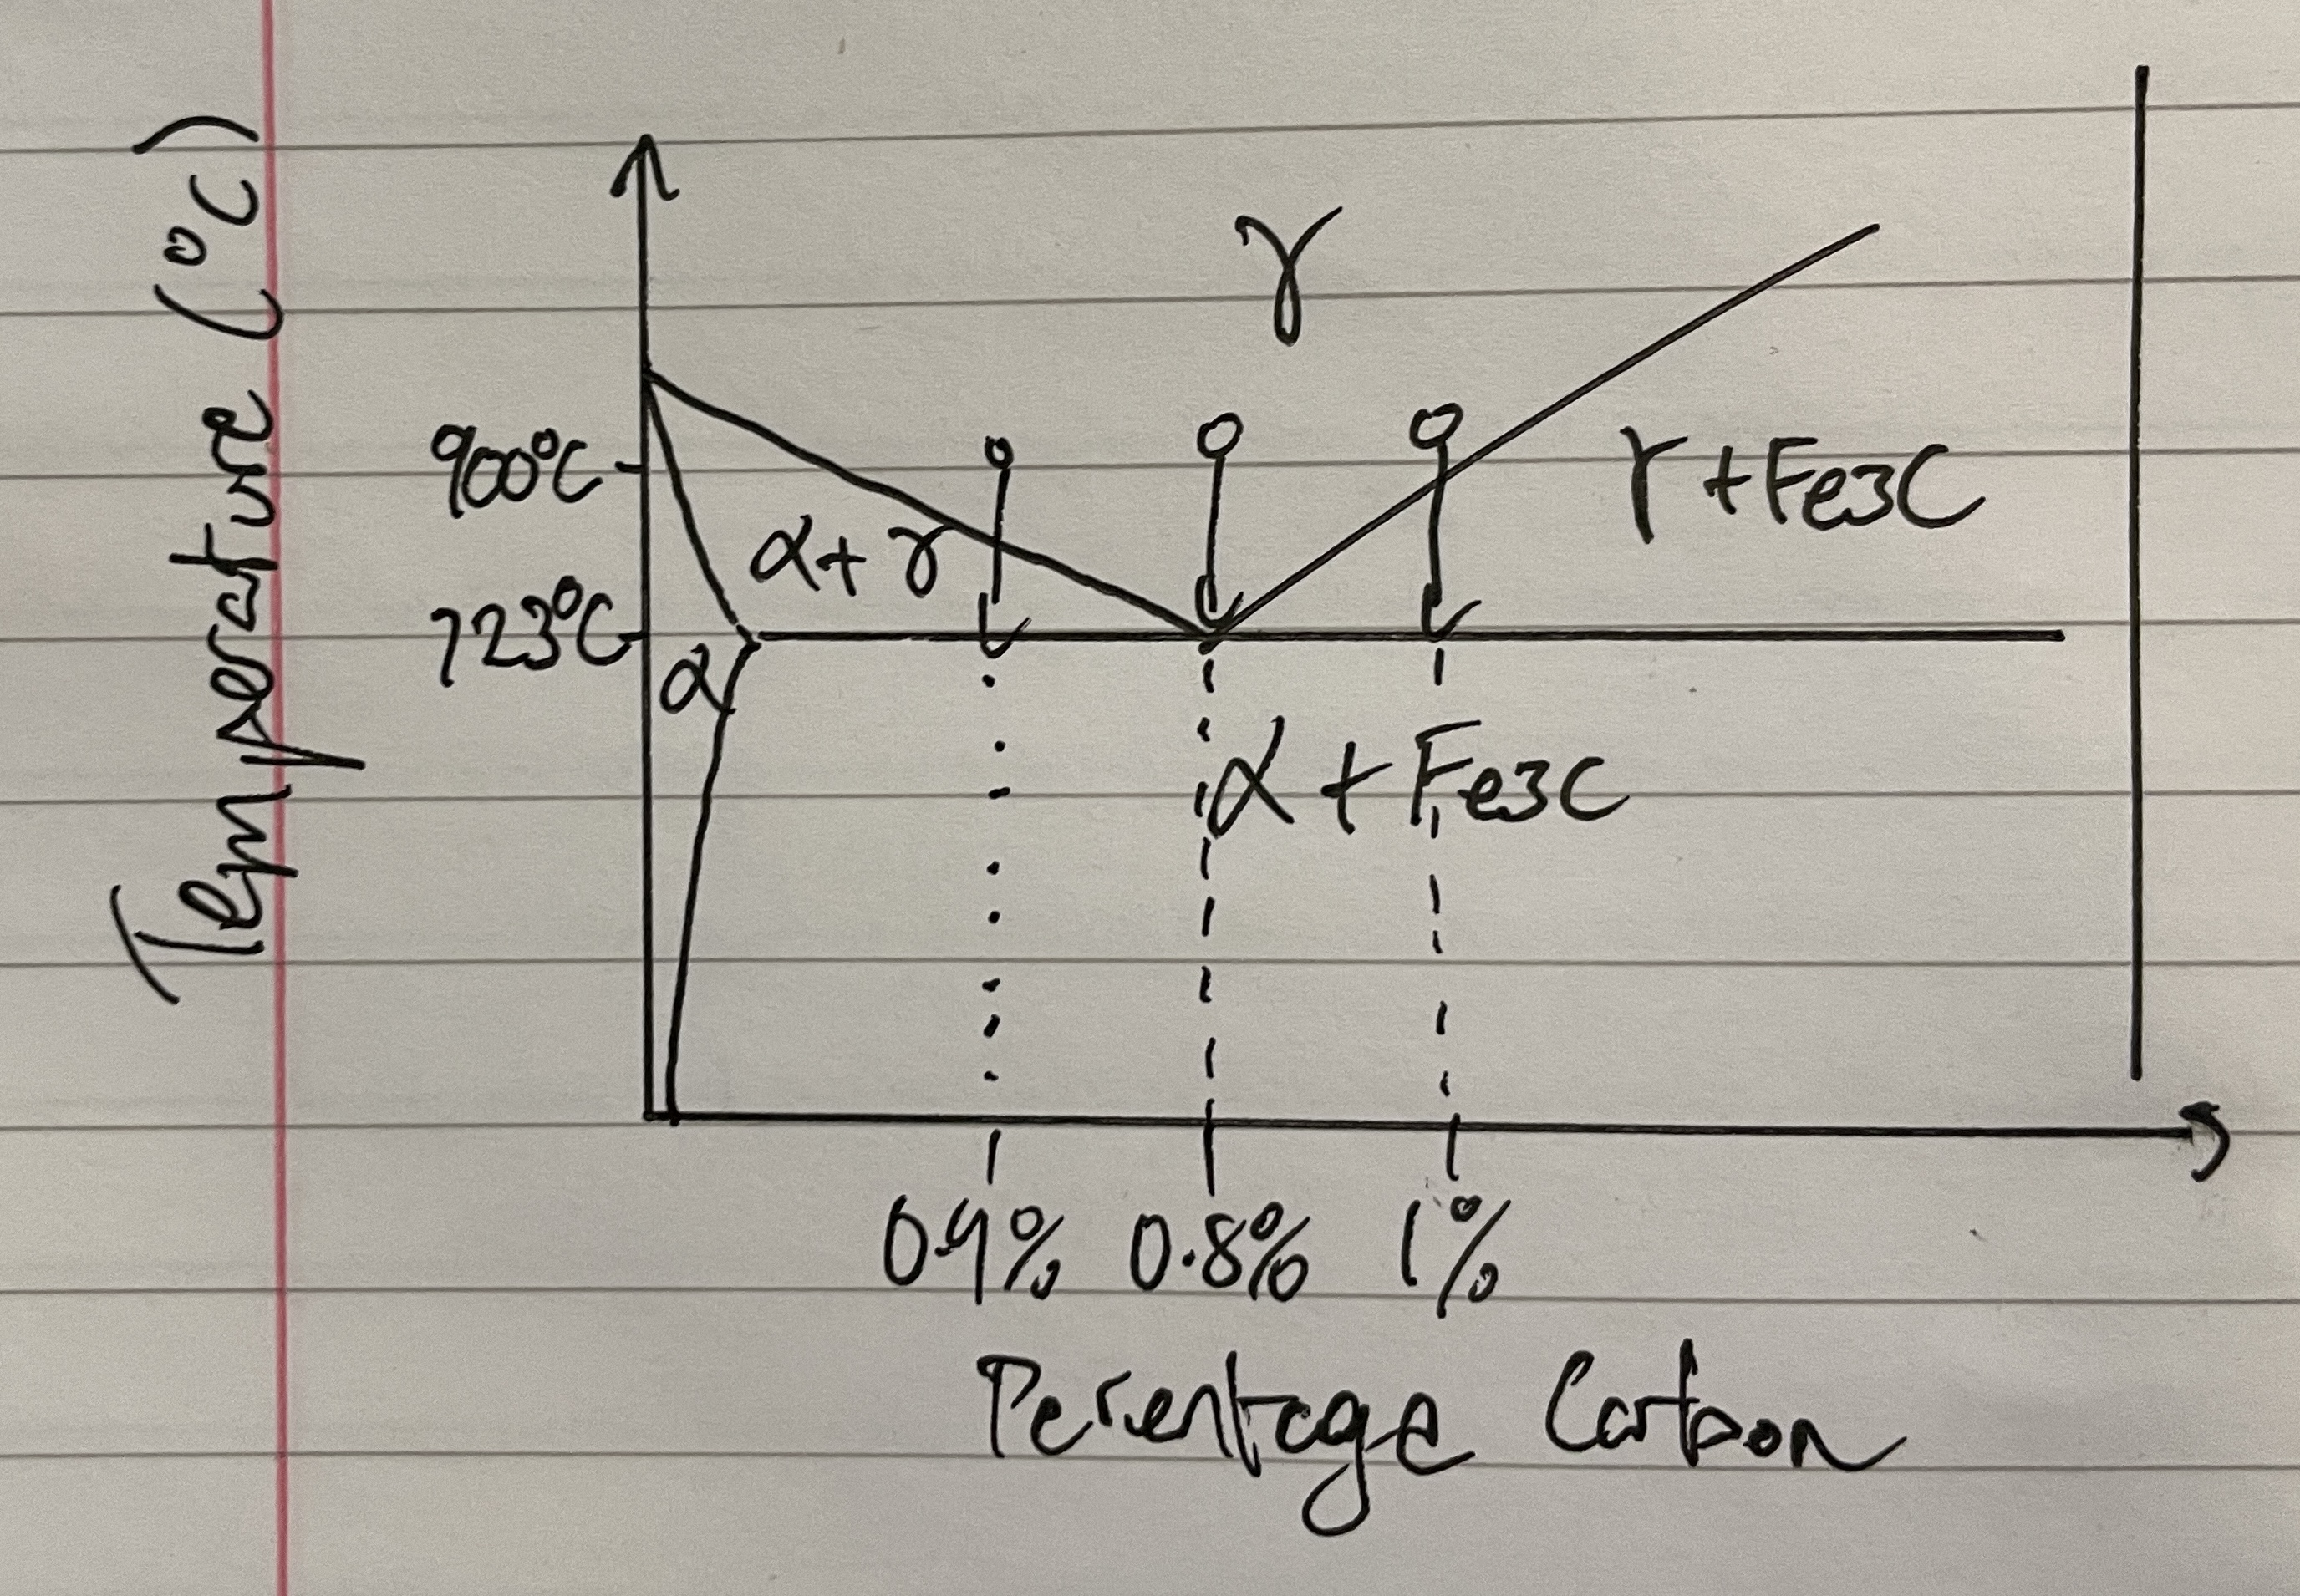
\includegraphics[width = 0.7\textwidth]{./img/q1b.jpg}
    \caption{Diagram showing cooling process.}
\end{figure}
\begin{figure}[H]
    \centering
    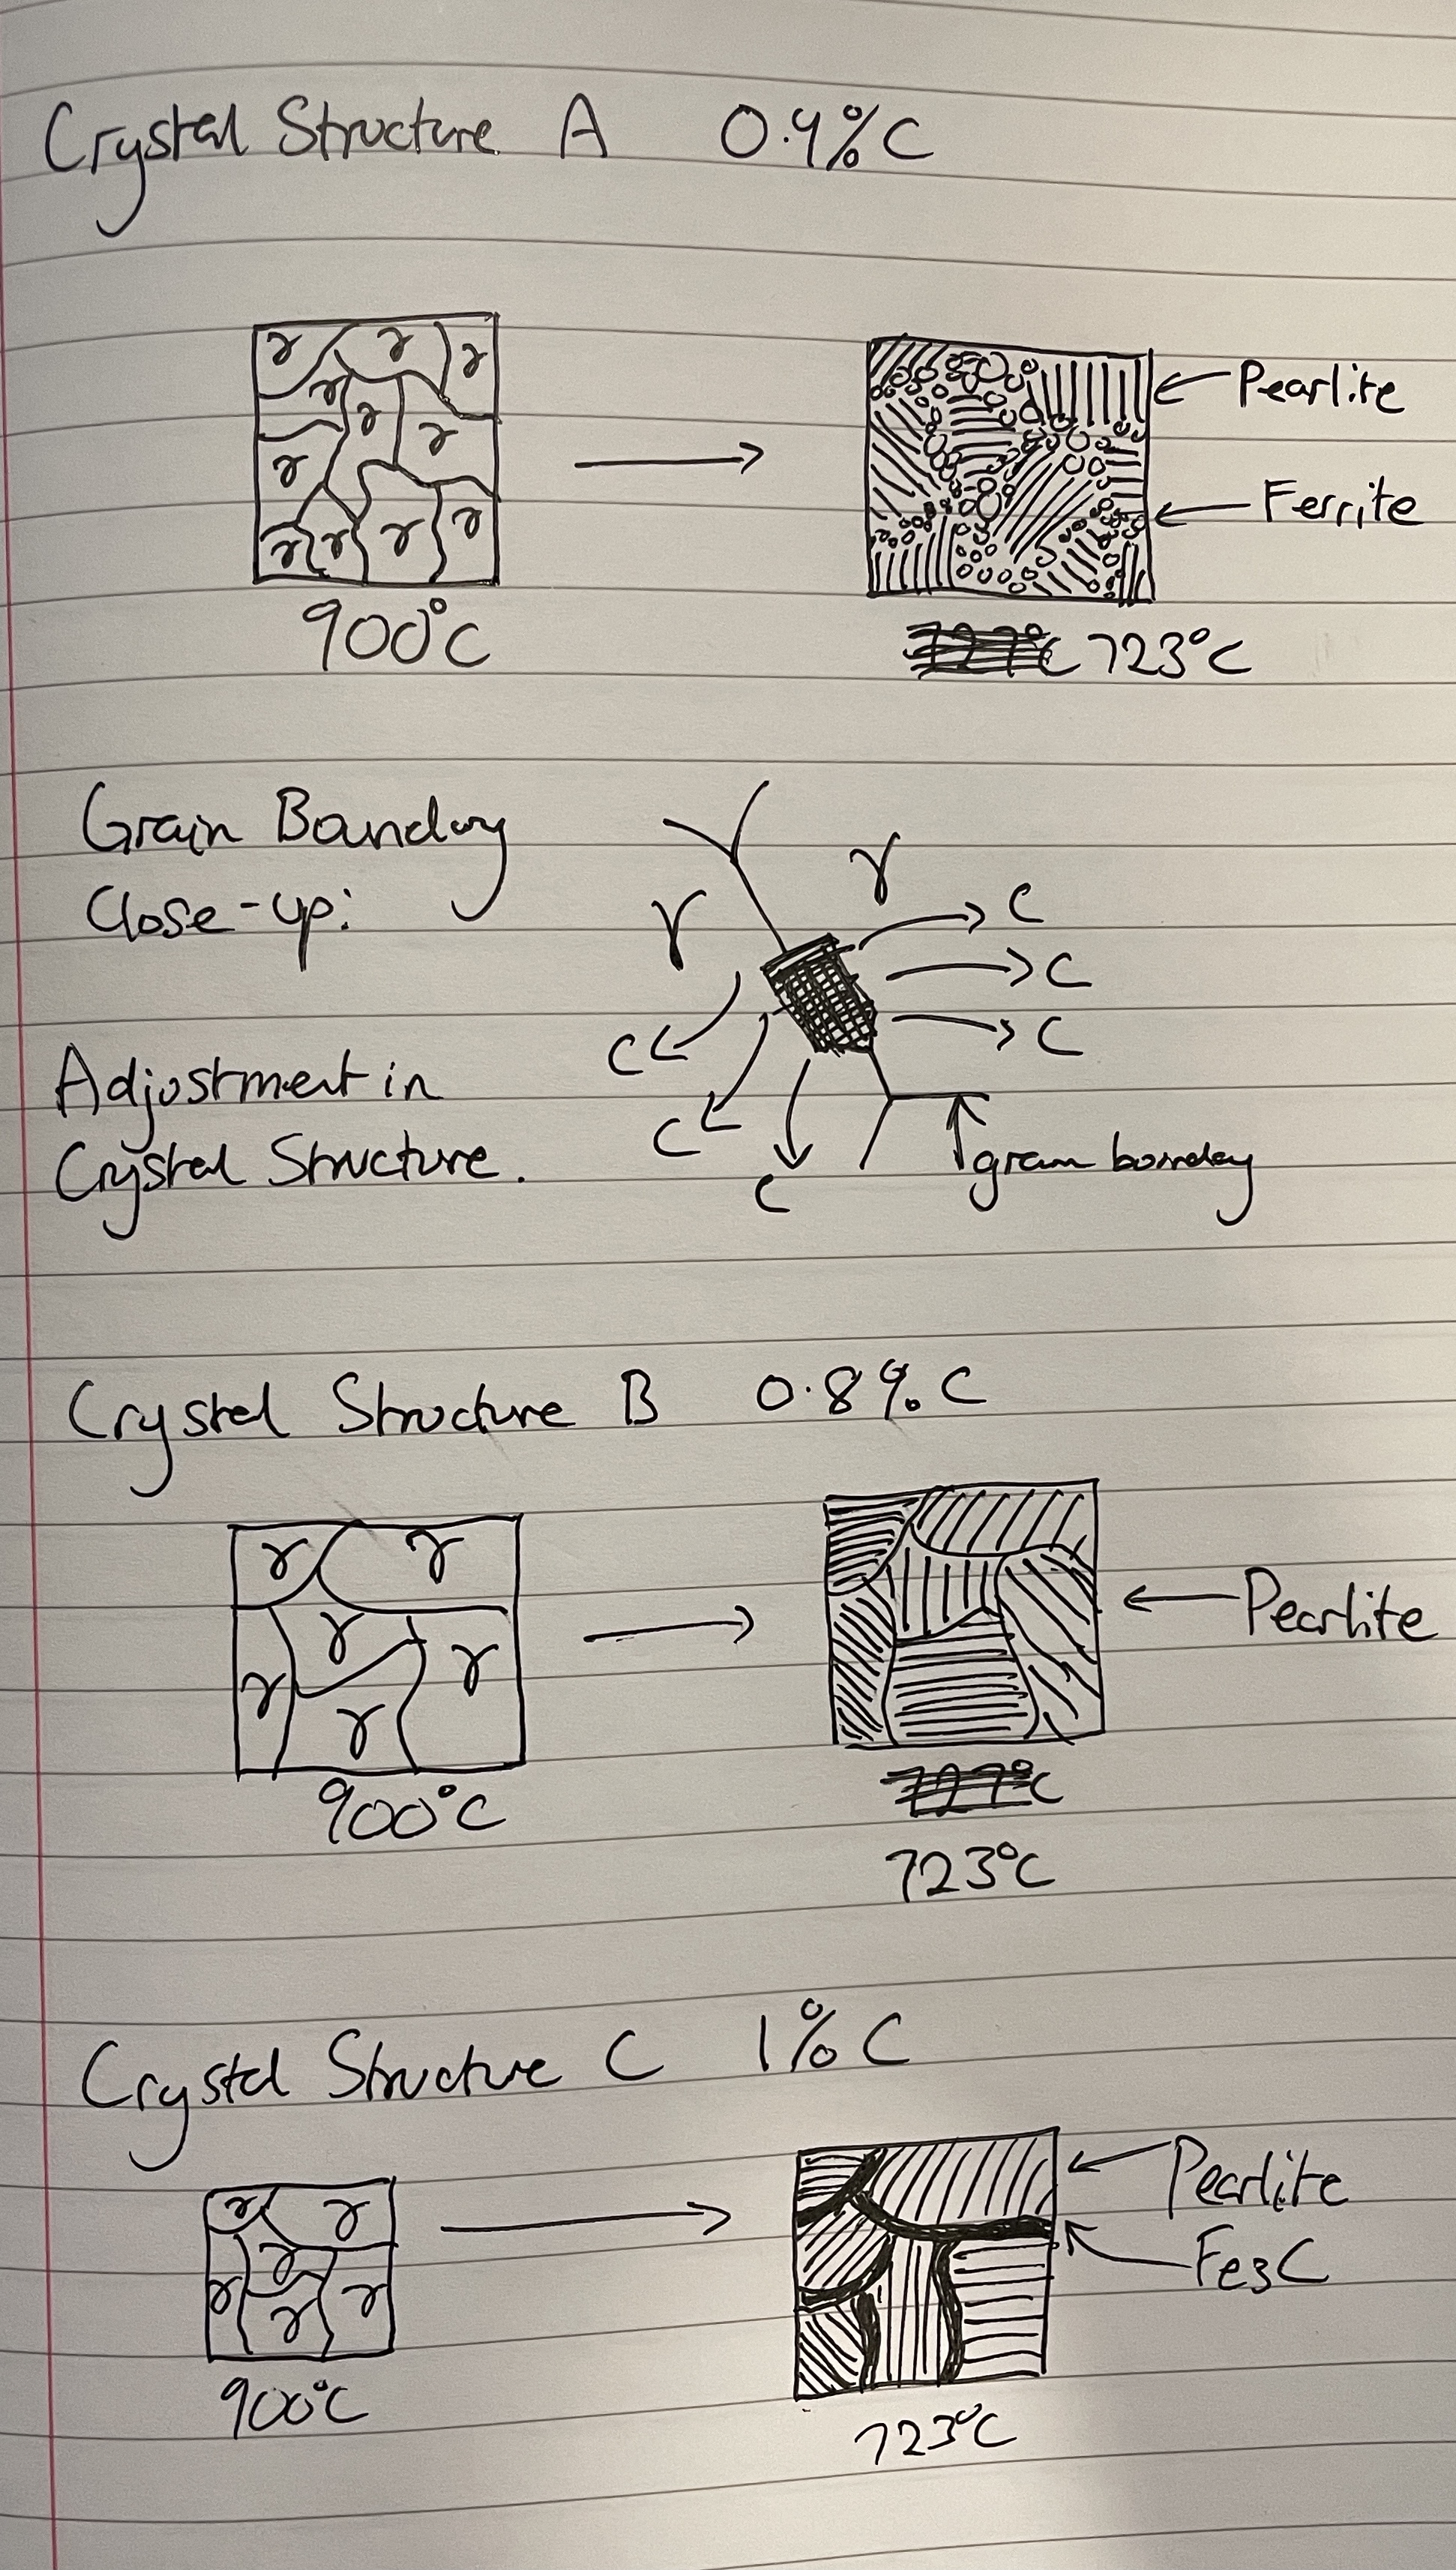
\includegraphics[height = 24cm]{./img/q1a.jpg}
    \caption{Diagrams showing how crystal structure changes with cooling from \SI{900}{\celsius} to \SI{723}{\celsius} for 0.4\%, 0.8\% and 1\% carbon content.}
\end{figure}

For 0.4\%, we can see the emergence of $\alpha$ forming at the grain boundary. This adjusts the crystal structure to form BCC areas and carbon must move away, enriching the $\gamma$ regions. This then converts the remaining $\gamma$ into pearlite as temperature decreases. With increasing carbon content, tensile strength increases as the amount of pearlite increases and the amount of $\alpha$ formed at the grade boundaries decreases. This increases tensile strength (until 0.8\% carbon content is reached) as dislocations become more difficult in the microstructure. 

For 0.8\% carbon content, the crystal structure forms a 100\% pearlite crystal structure. This structure is tough as the pearlite is saturated with carbon and there is a fine grain boundary with no formation of $\alpha$ or excess \ce{Fe3C}.

For 1\% carbon content, we see a conversion of some of the $\gamma$ into \ce{Fe3C} at the grain boundary, leading to embrittlement. We know that pearlite saturates at 0.8\% carbon content, so carbon moves away from the pearlite to form \ce{Fe3C} at the grain boundaries (which has a higher carbon content), coating the pearlite crystals. This has the consequence that due to the positioning and location of the primary \ce{Fe3C}, the whole steel exhibits the toughness of \ce{Fe3C}. This toughness is lower than that of 100\% pearlite and hence is undesirable for tensile applications and should be avoided. 
\begin{figure}[H]
    \centering
    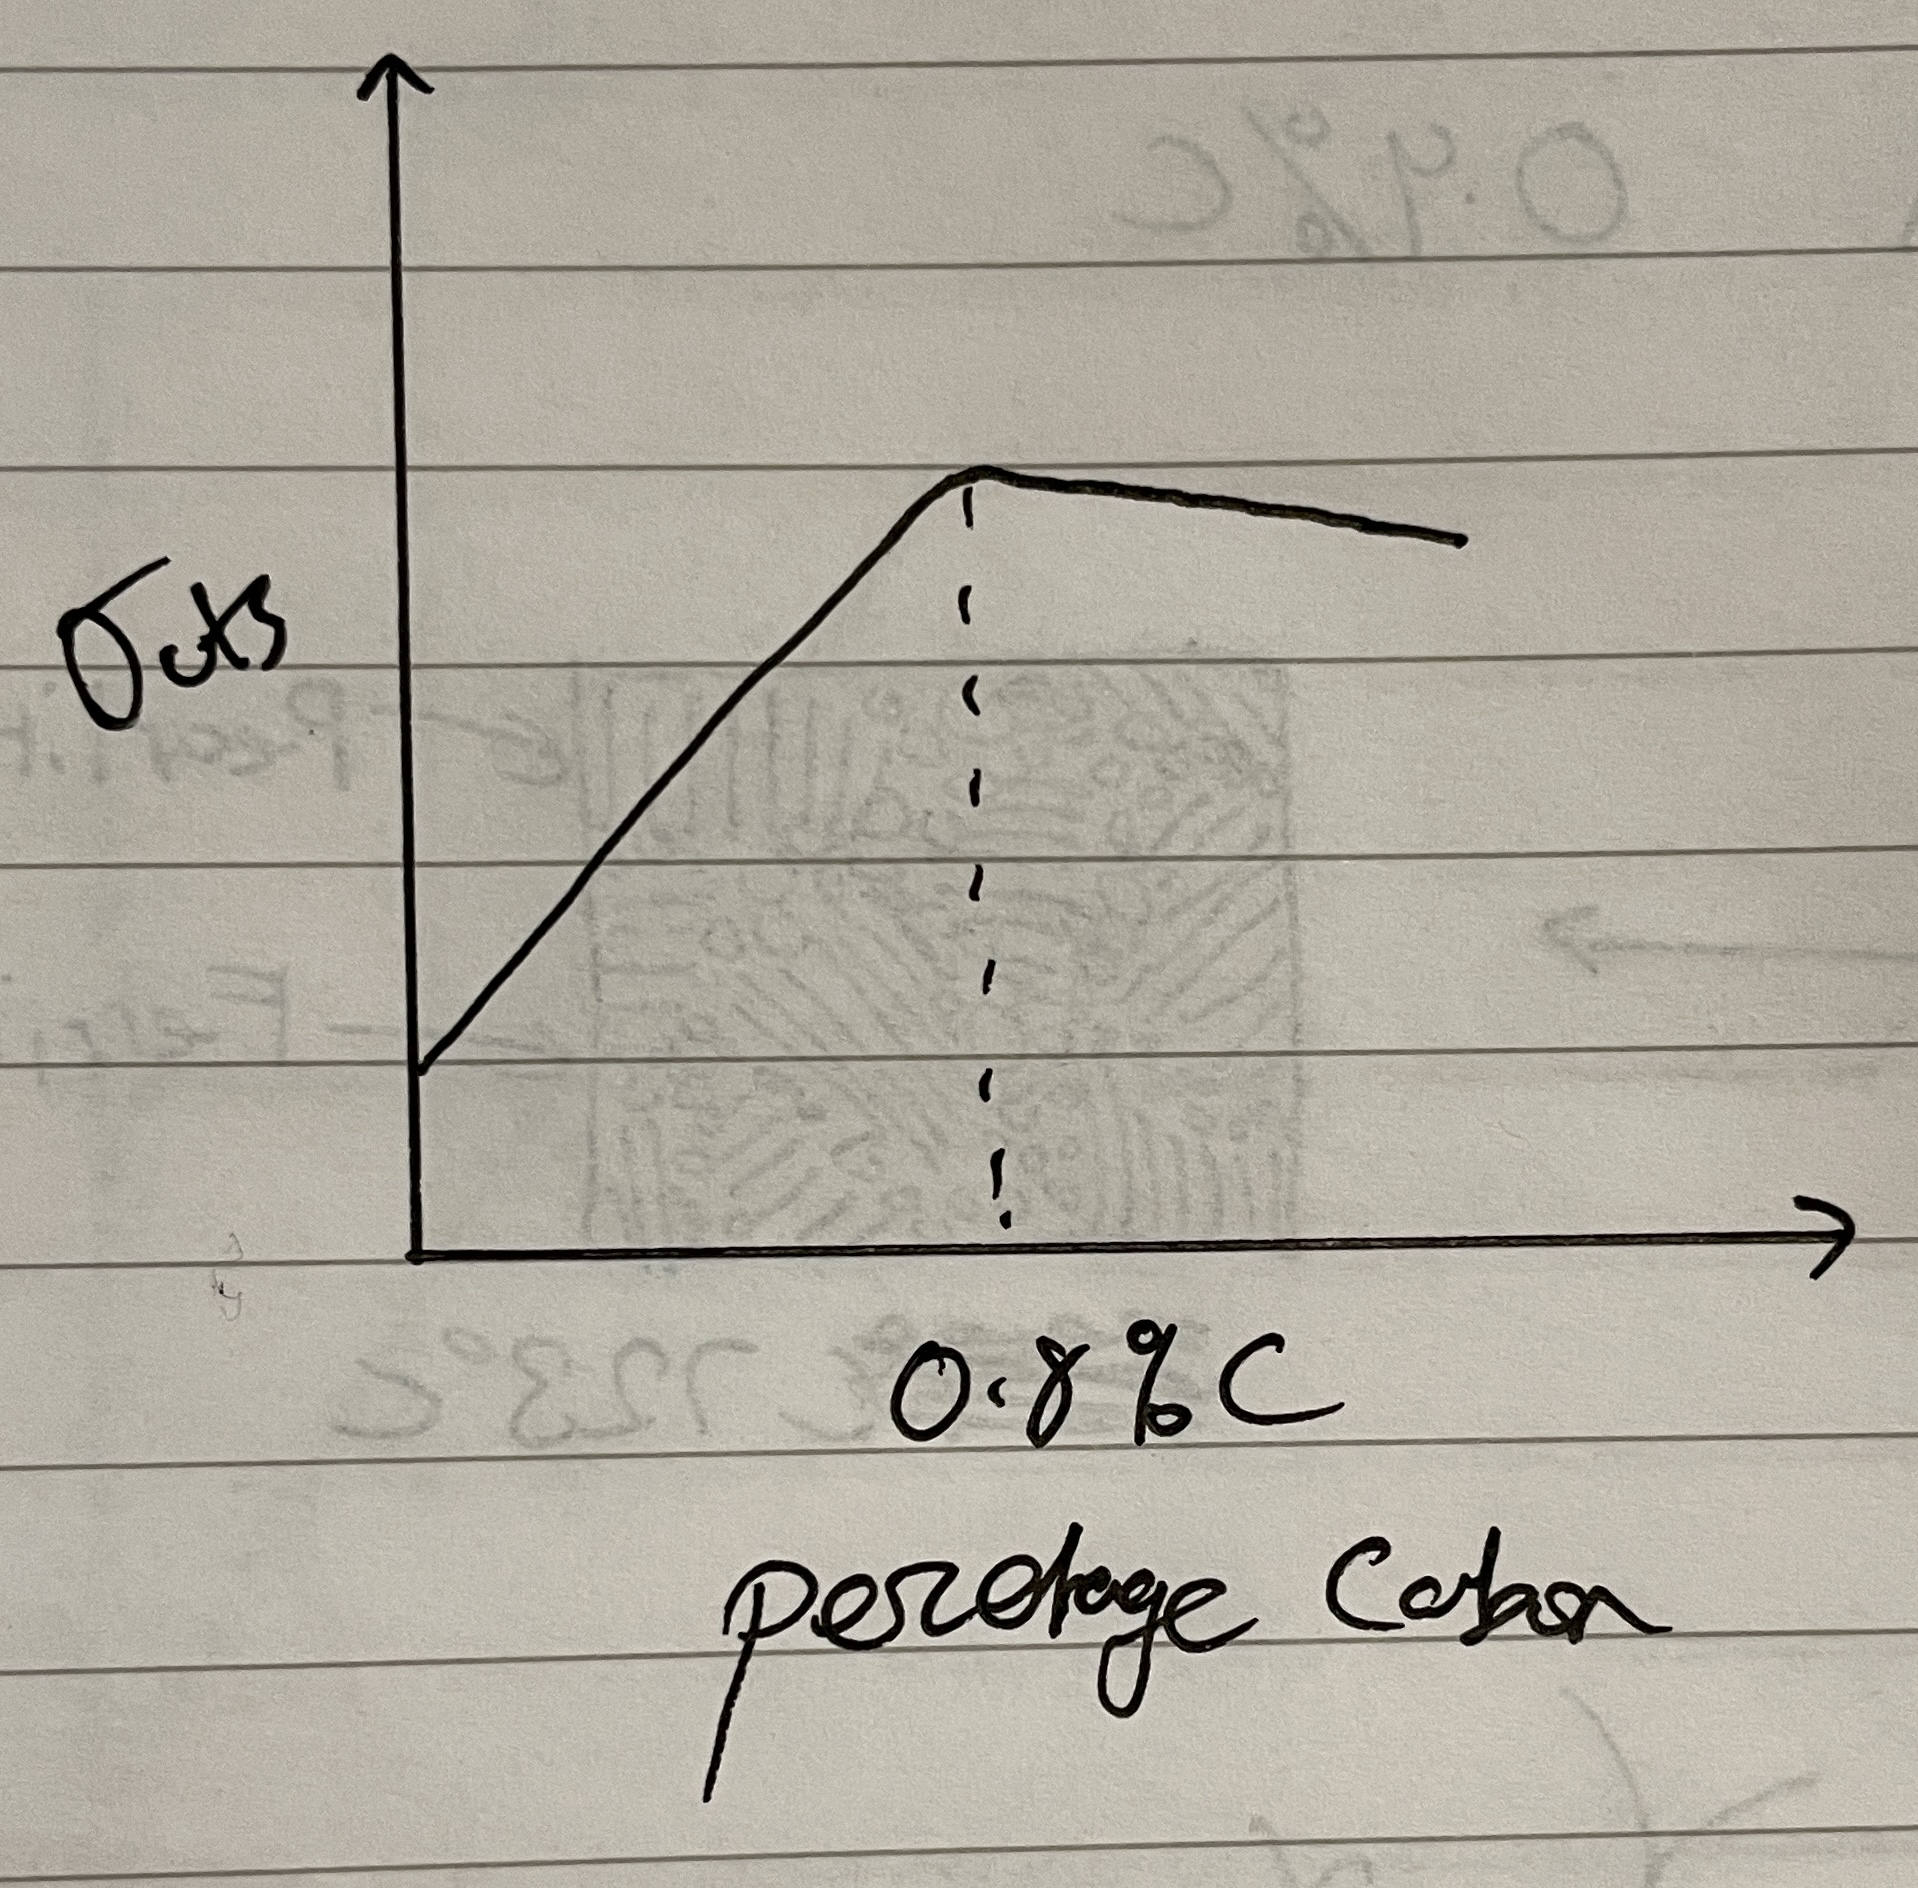
\includegraphics[width = 0.5\textwidth]{./img/q1c.jpg}
    \caption{Diagram showing how tensile strength varies with carbon content.}
\end{figure}
\section{Show that the area under the stress strain curve is equivalent to the elastic stored energy (in a stressed material). What part of the stress strain curve do you need?}
Let us define stress and strain. The equation for stress is given by:
\begin{equation}
    \sigma = \frac{F}{A}
\end{equation}
where $F$ is force and $A$ is the area over which that force is applied. The equation for strain is given by:
\begin{equation}
    \varepsilon = \frac{\dif x}{L}
\end{equation}
where $\dif x$ is the extension and $L$ is the original length of the test specimen. We can also define how elastic energy is stored as a function of the force applied over a distance:
\begin{equation}
    W = U = \int \left(F\right)\dif x\label{ss1}
\end{equation}
where $U$ is strain energy. We can use a mathematical trick to bring volume, area and length into \ref{ss1}:
\begin{equation}
    U = \frac{V}{A\cdot L} \int \left(F\right)\dif x
\end{equation}
Rearranging:
\begin{align}
    U &= \int\left(V\cdot \frac{F}{A}\cdot \frac{\dif x}{L}\right)\\
    U &= V\int\left(\sigma\right)\dif \varepsilon
\end{align}
Hence, we can derive strain energy per unit volume:
\begin{equation}
    \frac{U}{V} = \int \left(\sigma\right)\dif \varepsilon\label{ss2}
\end{equation}
\begin{figure}[H]
    \centering
    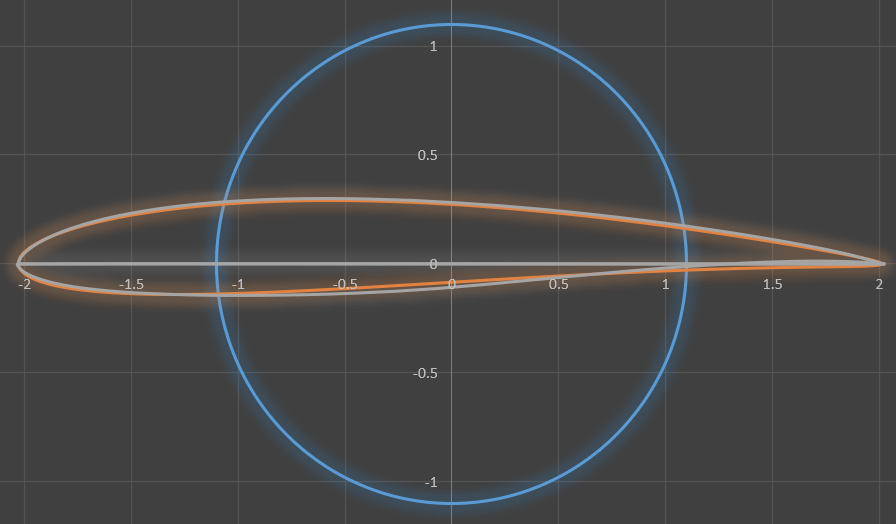
\includegraphics[width = 0.5\textwidth]{./img/q2a.jpg}
    \caption{Diagram showing a generic stress-strain graph, marked with limit of proportionality and yield point.}
\end{figure}
As we can see from the above graph, as long as the material is not extended past its yield point (limit of elasticity), the area under the graph describes the strain energy stored in the material. It is important that this limitation is recognised, as past the yield point, the material deforms plastically and cannot return to its original shape. Hence, we are only interested in the proportional region of the graph. Substituting Hooke's Law into \ref{ss2}:
\begin{align}
    \sigma &= E\varepsilon\\
    \frac{U}{V} &= \int\left(E\varepsilon\right)\dif \varepsilon\\
    \frac{U}{V} &= \frac{E\varepsilon^2}{2} = \frac{\sigma\varepsilon}{2}
\end{align}
This is the same as the triangular area under the stress-strain curve until the limit of proportionality is reached and is a good approximate for the area until the yield point.
\section{Why is martensite hard in steel?}
Martensite is formed when a steel is cooled rapidly, most often through quenching the specimen in oil or some other liquid. This rapid cooling process prevents the austentite structure to become another phase through diffusion easily. During cooling, austentite would like to turn into a lower energy state, such as ferrite/pearlite/\ce{Fe3C}, but during rapid cooling, this process cannot take place appropriately. As a result, the specimen can become martensite, in which we have a distorted BCC ferrite lattice structure \cite{b1}. The structure is distorted as the carbon has not been able to diffuse out of the structure and instead remains within the crystal structure, changing its shape.

\begin{figure}[H]
    \centering
    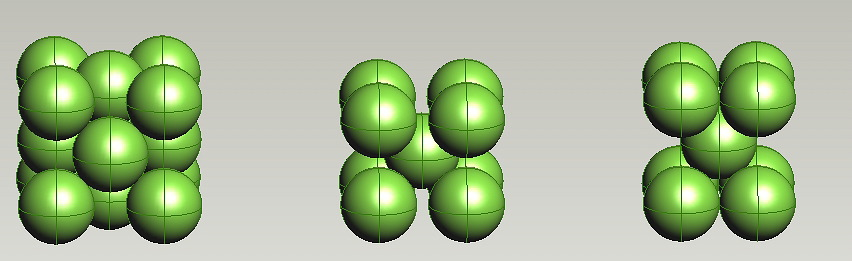
\includegraphics[width = 0.75\textwidth]{./img/q3a.jpg}
    \caption{Diagram showing FCC structure (left), BCC structure (centre) and BCT structure (right) \cite{b3}.}
\end{figure}
During the shearing process, the interstitial carbon remains in place and is unaffected by the neighbouring iron atoms. After cooling, these carbon atoms can no longer move and hence we form a structure which is slightly stretched. We cannot call this structure 'cubic' and hence this new structure is called body-centred-tetragonal. This BCT structure is different from a BCC structure in that we have lengthening in one axis only, the other two shorten \cite{b2}. This distortion is linked to the increase in the hardness of the material. All in all, we are left with a highly irregular and non-symmetric microstructure with high number of defects. Factors which contribute to the increased hardness of martensite relative to other structures include:
\begin{itemize}
    \item A large quantity of carbon remains in the solid solution. The carbon is interstitially spaced between the iron atoms and prevents dislocations from moving further. This strengthens the solution and contributes to the increase in hardness.
    \item The nature of a BCT structure has fewer slip systems as it is more irregular. This is due to the non-symmetric shape of the lattice structure and the interstitial carbon atoms arranged irregularly within the structure as well. This leads to a microstructure with a higher resistance to slip, increasing hardness.
    \item As martensite forms, the increase in volume associated with the formation of the BCT structure will create large residual stresses as crystals are forced to occupy a decreasing volume. This creates a very high dislocation density, increasing hardness.
\end{itemize}
\section{How can quench cracking be avoided from a design perspective?}
Quenching is used to change the mechanical properties of a sample. It is used to form martensite which has a high hardness but lacks in other mechanical properties, hence it is often followed up with a tempering process, to achieve more desirable properties. This process involves heating the sample to just above the recrystallisation temperature and then dipping the sample into a liquid such as mineral oil, rapidly cooling it. This prevents phase changes and diffusion, causing martensite to be formed from the surface inwards. 

During this quenching process, the metal will shrink in size. Hence, it is important that the sample is free from large defects such as microfractures, as these may propagate as the material changes shape. Defects act as a stress concentrator and the shrinking action brought out by quenching increases the internal stress of the specimen, potentially leading to fractures at those locations. This can be mitigated by controlling the rate of cooling. We can do this by changing the medium in which we are quenching our specimen to something with a lower specific heat capacity, as that would transfer energy away from the specimen more slowly. 

Since the geometry of the sample will determine where these stress concentrators are, it is important to have this in mind when designing our component for quenching. Things such as sharp corners or holes will create stress concentrators that may lead to quench cracking. The thickness of the sample will determine the depth to which martensite may form. Large changes in cross-section and thickness may bring about stress concentrations. Some ways of mitigating stress concentrations in our design include rounding edges and consistent shapes. Selecting a material with a higher carbon content may lead to an increased likelihood of failure. Hence, selecting an appropriate material and design is important for the quenching process

We must also ensure that our specimen is prepared appropriately for quenching. We should check the sample for pre-existing fractures or signs of failure. If the part has been machined, we should check to make sure that there are no imperfections/cracks, as these could act as stress concentrators. If the specimen is not heated to the correct temperature, quenching may not even form martensite. If the specimen is heated unevenly, quenching may cause imbalances and produce regions in which martensite has formed and areas in which it has not. These imperfections can bring about defects which may cause failure. To conclude, design the sample with quenching in mind and perform checks and take preventative measures to ensure that failure does not occur.
\begin{thebibliography}{00}
    \bibitem{b1} H. Föll (Iron, Steel and Swords script), "Be Cool! 8.4.1 Martensite", \url{https://www.tf.uni-kiel.de/matwis/amat/iss/kap_8/backbone/r8_4_1.html#:~:text=Martensite%20in%20steel%20is%20only,transformation%3B%20it%20is%20rather%20soft.} Accessed 25/04/21 23:45
    \bibitem{b2} Miles Free, "Martensite- Five Facts", March 15, 2011: \url{https://pmpaspeakingofprecision.com/tag/why-martensite-is-harder-than-austenite/} Accessed: 25/04/21 23:58
    \bibitem{b3} Face-centred cubic, body-centred cubic and body-centred tetragonal arrangements of iron atoms. \url{https://www.phase-trans.msm.cam.ac.uk/2007/Atoms/Atoms-Pages/Image1.html} Accessed 26/04/21 00:09
\end{thebibliography}
\end{document}